\documentclass{scrreprt}
\usepackage{graphicx}
\usepackage{subcaption}
\usepackage{float}
\usepackage{amsmath}
\usepackage{listings}
\usepackage{color}
\usepackage{tikz}
\usepackage{circuitikz}

\title{RC Circuit Response to \\ Step, Pulse, and Square Inputs}
\author{Jnanesh Sathisha Karmar - EE25BTECH11029 \\ Vivek Kumar - EE25BTECH11062}
\date{January 30, 2026}

\definecolor{lbcolor}{rgb}{0.96,0.96,0.863} 

\lstset{basicstyle=\ttfamily, keywordstyle=\rmfamily\bfseries, backgroundcolor=\color{lbcolor}}

\begin{document}

\maketitle

\section{RC circuit diagram}

\begin{circuitikz}[american voltages]
	\draw (0, 3) 
        to[V, l_ = $V_s$](0, 0);
    \draw (0, 3)
	    to[R, l = $820 \Omega$](3, 3)
        to[C, l_ = $1 \mu F$, v^ = $V_{out}$](3, 0)
        -- (0, 0)
        node[ground]{};
\end{circuitikz}

Here is the diagram of a RC circuit. RC circuits are low-pass filter circuits. The value of resistance and capacitance was chosen to be $R = 820 \Omega$ and $C = 1 \mu F$. We will now observe the behaviour and relation of $V_{out}$ for different $V_s$. We will observe the response of different step, pulse and square inputs.

\section{Step Input (Single Event)}

\subsection{Charging Response}

\subsubsection{Experimental Results}

\begin{figure}[H]
    \centering
    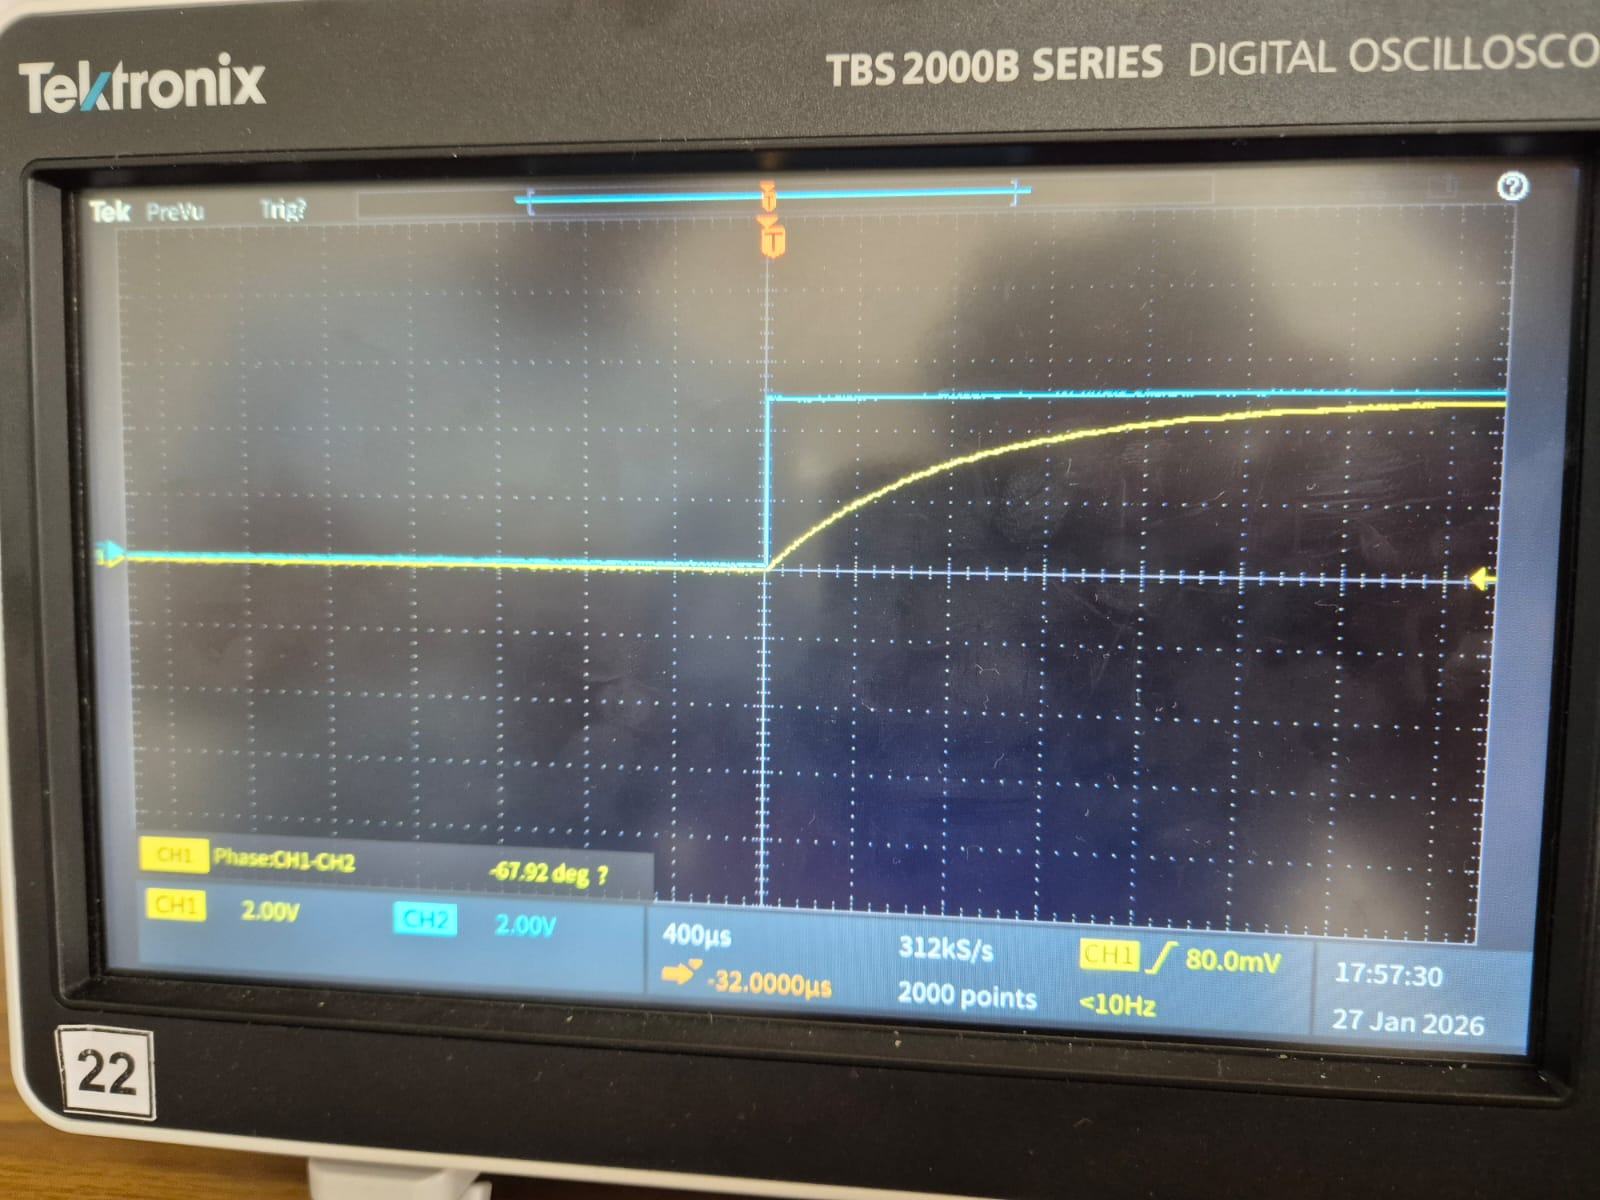
\includegraphics[width=0.8\linewidth]{figs/StepSignal_charging.jpeg}
    \label{fig:dso-stepsignal(charging)}
\end{figure}

\subsubsection{Signal Information}

Blue Waveform (CH2): Step input (square rise edge). A step input of the form $V_s = 5u(t)$ was applied. This input signal could be generated by the AFG by applying a pulse signal of very very large width. \\
Yellow Waveform (CH1): Capacitor charging curve. This is the output and the voltage across the capacitor. We can see that this is the type of response we get for a step signal.\\

CH1 scale: $2.00\,\text{V/div}$

CH2 scale: $2.00\,\text{V/div}$

Time scale: $400\,\mu s/\text{division}$

\subsection{Theoretical response}

For a step input voltage \quad  $V_s(T):$ \quad $V_C(t) = V_s\left(1 - e^{-t/RC}\right)$

\subsubsection{Computing time constant from measurement}

For computing the time constant, we look at the charging waveform.

We compute time constant by measuring the time voltage across resistor takes to reach the voltage at one time constant.

Here $V_c(t)$ is the voltage across the capacitor at time t.

At one time constant $t = \tau = RC$:
\begin{align}
V_C(\tau) = V_s(1 - e^{-1}) = 0.632V_s \\
V_C(\tau) = 0.632 \times 5 = 3.16V
\end{align}

From the graph we can take around 8 small divisions (1.6 divisions) to find the corresponding time. We find that the corresponding time is close to $800\mu s$ due to it being around 2 time divisions away from the axis.
\begin{align}
t \approx 800 \mu s
\end{align}
This aligns with the actual value of resistances and capacitances we took. The theoretical value of t is $t = 820 \mu s$. The error is less than 3\%.

\subsubsection*{Verification - Hand Calculation}
When the input is removed: \quad $V_C(t) = V_0 e^{-t/RC} $ \\
Substituting $RC = 0.82\,ms$:
\begin{equation}
V_C(t) = V_0 e^{-t/0.82ms}
\end{equation}
At $t = \tau$:
\begin{align}
V_C = 0.368V_0
\end{align}
At $t = 5\tau = 4.1\,ms$, the capacitor is almost fully discharged.

\subsubsection{Verification Using $2\tau$}

The theoretical time constant of the RC circuit is:

\[
\tau = RC = 820 \times 1\times10^{-6} = 0.82\,ms
\]

Hence,

\[
2\tau = 2 \times 0.82 = 1.64\,ms
\]

For a step input, the capacitor charging equation is:

\[
V_C(t) = V_s\left(1 - e^{-t/\tau}\right)
\]

At \(t = 2\tau\):

\[
V_C(2\tau) = V_s\left(1 - e^{-2}\right)
\]

\[
V_C(2\tau) = V_s(1 - 0.135)
\]

\[
\boxed{V_C(2\tau) \approx 0.865\,V_s}
\]

From the experimental waveform, the capacitor voltage at approximately
\(t = 1.64\,ms\) was observed to be close to \(86.5\%\) of the final value.

Thus, the experimental result agrees well with the theoretical prediction, verifying the step response of the RC circuit.


\section{Pulse Input (Single Event)}

\subsection{Short pulse ($T \ll RC$)}
\subsubsection{Signal Information}
\subsubsection{Hand Calculation}
\begin{align}
T_p \ll 820\mu s
\end{align}
Peak capacitor voltage:
\begin{equation}
        V_{max} = V_s\left(1 - e^{-T/RC}\right) \label{eq:vmax}
\end{equation}
For $T \ll RC$:
\begin{align}
V_{max} \approx \frac{T}{RC}V_s
\end{align}

\subsection{ Pulse width ($T \approx RC$)}
\subsubsection{Signal Information}
\subsubsection{Hand Calculation}
From \eqref{eq:vmax}, it follows that
\begin{align}
T \approx 820\mu s \\
V_{max} = V_s(1 - e^{-1}) = 0.632V_s
\end{align}

\subsection{Long Pulse $T \gg RC$}
\subsubsection{Signal Information}
\subsubsection{Hand Calculation}
From \eqref{eq:vmax}, it follows that
\begin{align}
T \gg 820\mu s \\
V_{max} \approx V_s
\end{align}

We notice that, the capacitor charges almost completely during ON time and discharges exponentially during OFF time.

\section{Square-Wave Input (Transient and Steady-State)}
\subsection{$RC \gg T$}

\begin{align}
T \ll RC \\
T \ll 0.82\,ms
\end{align}

\subsubsection*{Hand Calculations}

For capacitor charging:

\begin{equation}
V_C(t) = V_i + (V_f - V_i)\left(1 - e^{-t/RC}\right)
\end{equation}

Since $t \le \frac{T}{2} \ll RC$,

\[
\frac{t}{RC} \ll 1
\]

Using approximation:

\[
e^{-t/RC} \approx 1 - \frac{t}{RC}
\]

\[
V_C(t) \approx V_i + (V_f - V_i)\frac{t}{RC}
\]

\subsubsection*{Inference}

The capacitor voltage varies almost linearly with time.  
Hence, the output waveform is approximately triangular.

\[
\boxed{\text{RC circuit behaves as an integrator}}
\]

\subsection{Case 2: $RC \approx T$}

\[
T \approx RC = 0.82\,ms
\]

\subsubsection*{Hand Calculations}

During the charging interval:

\begin{equation}
V_C(t) = V_s\left(1 - e^{-t/RC}\right)
\end{equation}

At the end of half cycle:

\[
t = \frac{T}{2} \approx \frac{RC}{2}
\]

\[
V_C = V_s\left(1 - e^{-0.5}\right)
\]

\[
V_C \approx 0.393V_s
\]

During discharge:

\begin{equation}
V_C(t) = V_0 e^{-t/RC}
\end{equation}

At $t = \frac{T}{2}$:

\[
V_C = V_0 e^{-0.5} \approx 0.607V_0
\]

\subsubsection*{Inference}

The capacitor partially charges and partially discharges in each cycle.  
Both transient and steady-state components are present.

\[
\boxed{\text{Maximum transient behavior is observed}}
\]

THIS IS CASE THREE
\subsection{Case 3: $RC \ll T$}

\[
T \gg RC
\]

\[
T \gg 0.82\,ms
\]

\subsubsection*{Hand Calculations}

During ON time:

\[
t = \frac{T}{2} \gg RC
\]

\[
e^{-t/RC} \approx 0
\]

\[
V_C \approx V_s
\]

During OFF time:

\begin{equation}
V_C(t) = V_s e^{-t/RC}
\end{equation}

For $t \gg RC$:

\[
V_C \approx 0
\]

\subsubsection*{Inference}

The capacitor fully charges and discharges within each cycle.

\[
\boxed{\text{Output closely follows the input waveform}}
\]


\end{document}

